\chapter{Tutorial básico de uso do aplicativo VidAnalysis}
\label{sec:vidanalysis}
\vspace{-0.7cm}

 
VidAnalysis é um aplicativo para análise física de movimentos em vídeos muito fáceis de usar.
O aplicativo é compatível com Android e pode ser baixado gratuitamente em \href{https://play.google.com/store/apps/details?id=com.vidanalysis.free}{\textcolor {blue}
{https://play.google.com/store/apps/details?id=com.vidanalysis.freey}}, ou simplesmente pesquise no Google Play com o nome VidAnalysis free. O aplicativo possui apenas uma versão em inglês, mas devido à simplicidade de seu uso, ele não representa nenhum problema.

Para realizar a coleta de dados das posições do objeto gravado no vídeo, siga as etapas abaixo:

\underline{\bf Passo 1:} {\bf Abertura do vídeo a ser analisado}\\


Primeiro, temos que gravar um vídeo ou importar um existente. Se você decidir importar um vídeo, ``click'' no sinal de adição mostrado com uma seta preta na Figura~\ref{apendice1c}. Como o aplicativo VidAnalysis suporta apenas formatos de vídeo com extensão ``mp4'' é recomendável gravar  diretamente dentro do aplicativo, escolhendo a opção marcada pela seta vermelha na Figura~\ref{apendice1c}.
Ao capturar vídeos para análise, é importante que a câmera esteja fixa, que o movimento esteja dentro do plano da câmera, e que no vídeo gravado apareça alguma referencia de 
um comprimento conhecido, por exemplo de uma régua. 

\begin{figure}[h!]
\centering
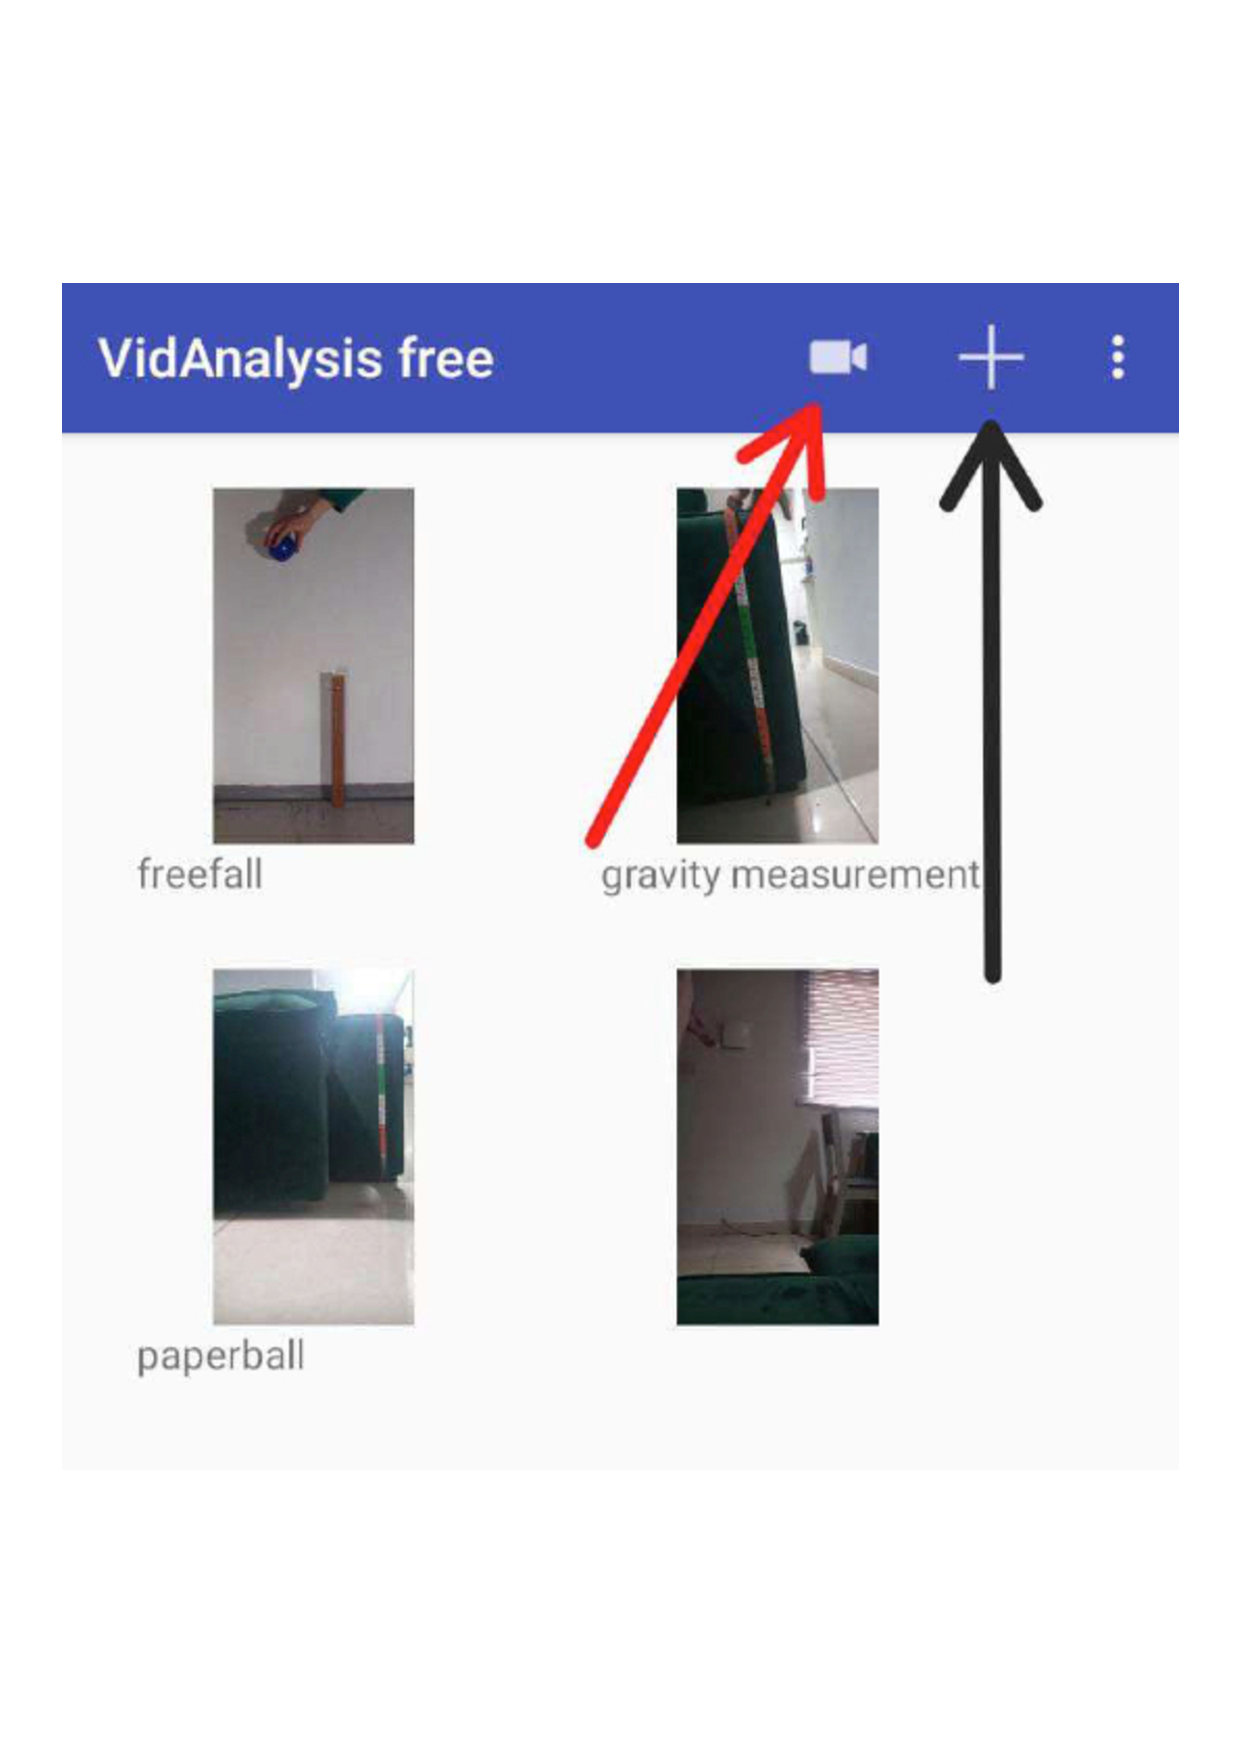
\includegraphics[width=8cm]{Figuras_exp3/imagenapendicec1.pdf}
\caption{\label{apendice1c} Menu do aplicativo VidAnalysis.}
\end{figure}

\vskip 0.5cm
\underline{\bf Passo 2:} {\bf Calibração}\\


Para começar a análise do movimento do objeto primeiramente  
selecionamos o vídeo no reprodutor e será aberta a primeira imagem dele como se mostra na Figura \ref{apendice2c}. É importante avançar o vídeo nessa tela, para começar a coleta de dados da trajetória do objeto diretamente no momento em que o movimento  começa, para isso fazemos ``click'' no botão mostrado pela seta verde na Figura~\ref{apendice2c} até avançarmos ao quadro do vídeo que interessa. Fazendo ``click'' nos três pontos indicado pela seta azul na Figura~\ref{apendice2c}, conseguimos ocultar o menu em preto, para uma melhor visualização do vídeo.

\begin{figure}[h!]
\centering
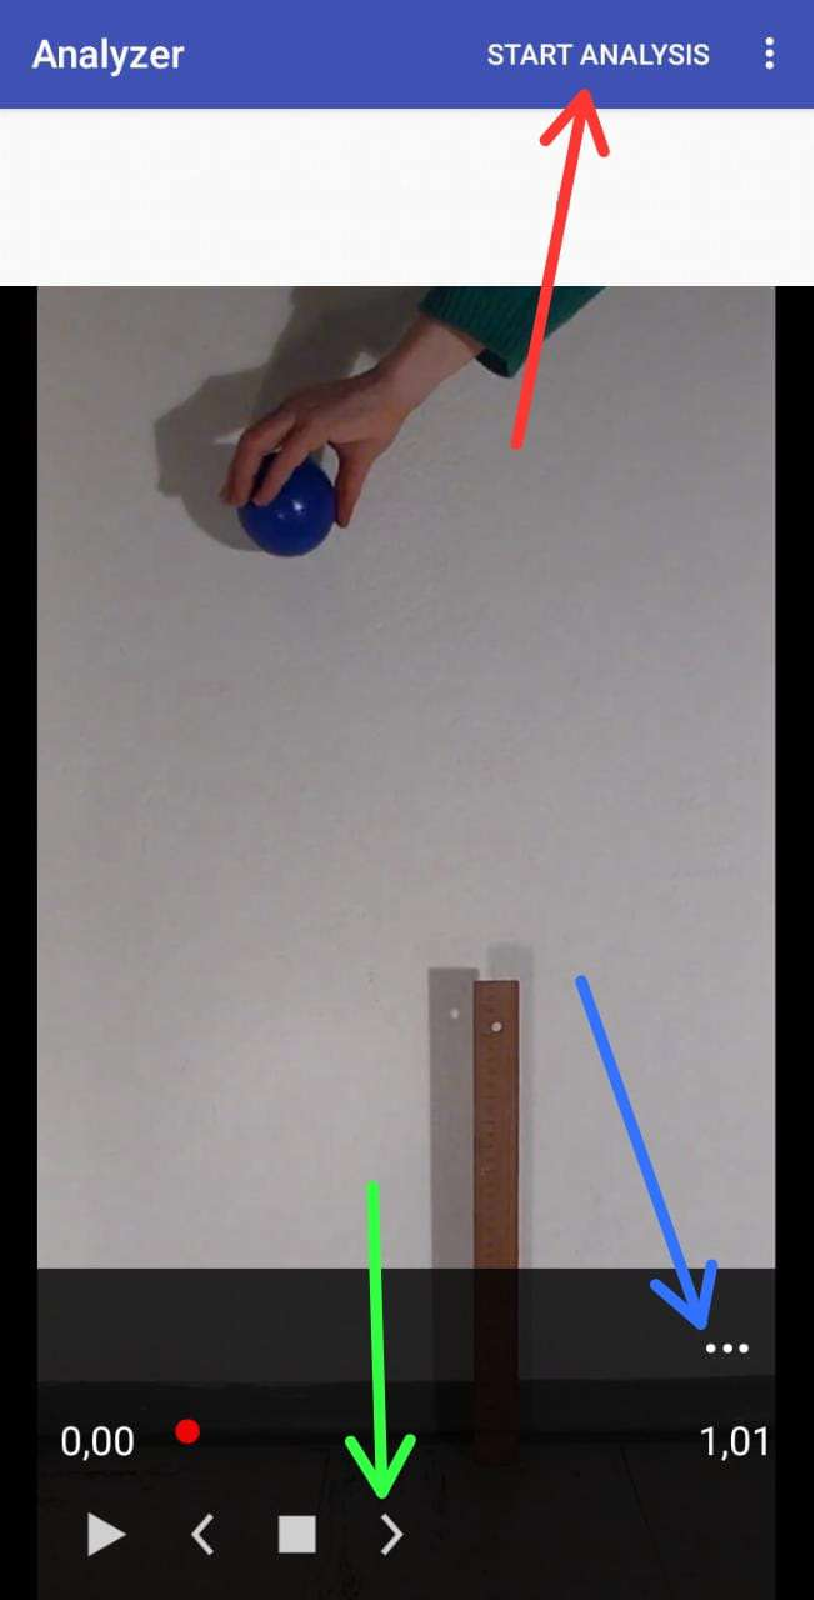
\includegraphics[width=8cm]{Figuras_exp3/imagenapendicec2.pdf}
\caption{\label{apendice2c} Reprodutor de video do aplicativo VidAnalysis.}
\end{figure}

Antes da coleta de dados deve primeiro calibrar qual é a escala de comprimentos que será usada pelo aplicativo. Para isso, fazemos ``click'' na aba ``start analysis''  no canto superior direito na Figura \ref{apendice2c}. Agora temos que marcar o comprimento conhecido.
 Ao fazer ``click no ponto inicial do comprimento conhecido, na tela esse ponto será marcado com uma cruz azul. Em seguida, deve fazer “click“ novamente no ponto final do comprimento conhecido e outra cruz azul indicará esse ponto. Após finalizar essa segunda marcação abrirá imediatamente uma janela solicitando o tamanho conhecido, como mostramos na Figura~\ref{apendice3c}. A legenda em inglês na janela pergunta ``Qual é o comprimento real disto em metros'' (``How many meters is this in real'' em inglês). É importante saber que a unidade a ser usada pelo aplicativo para comprimentos é sempre metros portanto as velocidades serão em metros por segundo por exemplo.
 
\begin{figure}[h!]
\center
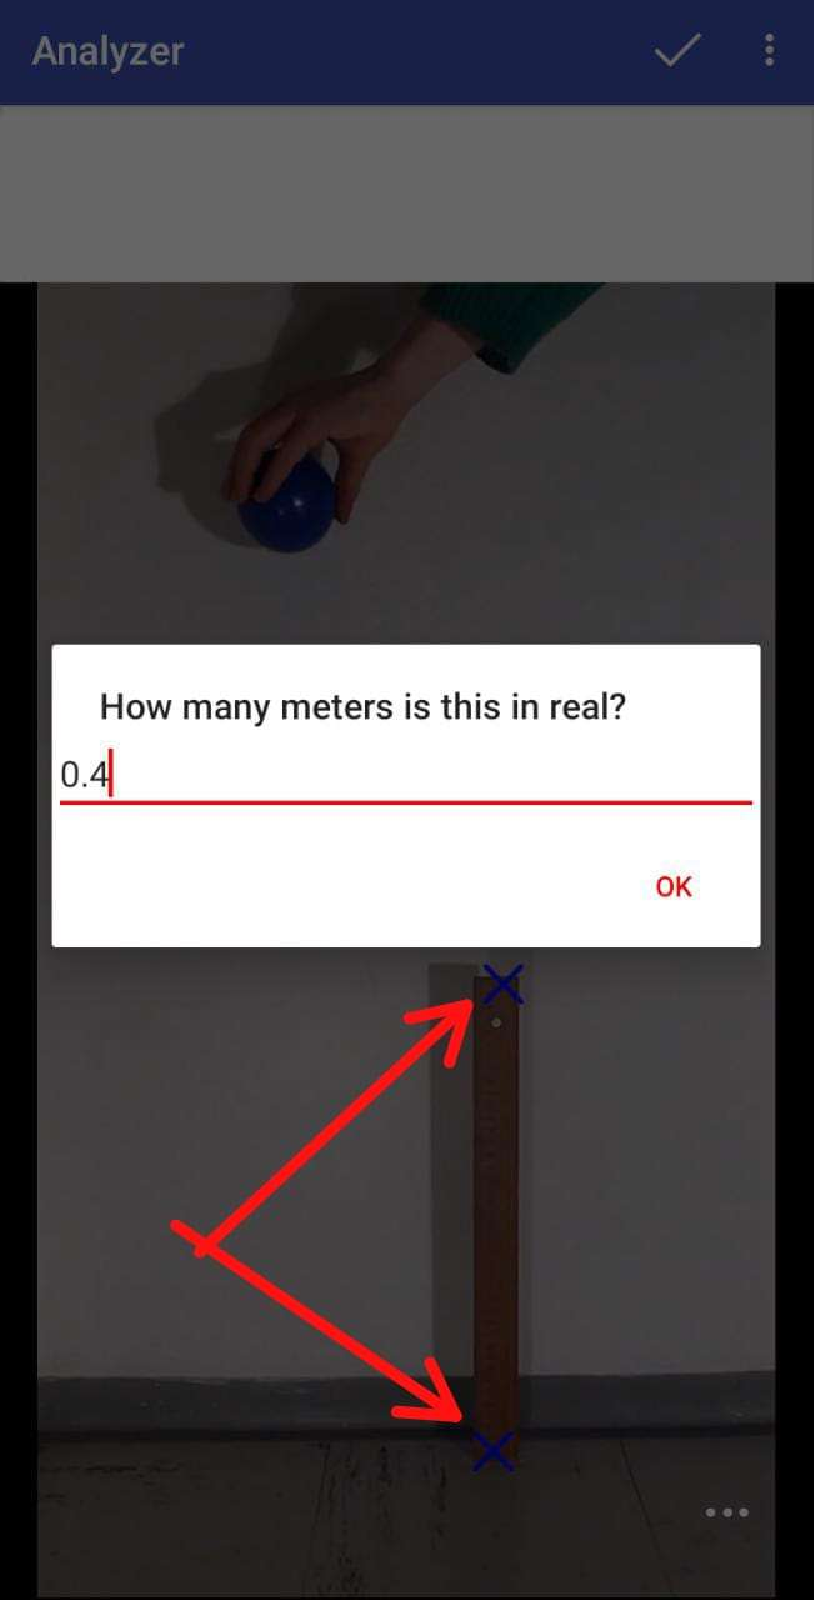
\includegraphics[width=8cm]{Figuras_exp3/imagenapendicec3.pdf}
\caption{\label{apendice3c} Escolha da escala de comprimentos no reprodutor de vídeo do aplicativo VidAnalysis, a ser usado na tomada de dados dos pontos da trajetória do objeto.}

\end{figure}
Após dar ``ok'' na janela da escala aparecerá um sistema de eixos coordenados cuja origem devemos estabelecer (ver Figura  \ref{apendice4c}). Em geral, é uma boa ideia posicionar a origem de coordenadas de tal maneira que as coordenadas da posição do objeto sempre tenham o mesmo sinal ao longo da trajetória.

\begin{figure}[h!]
\centering
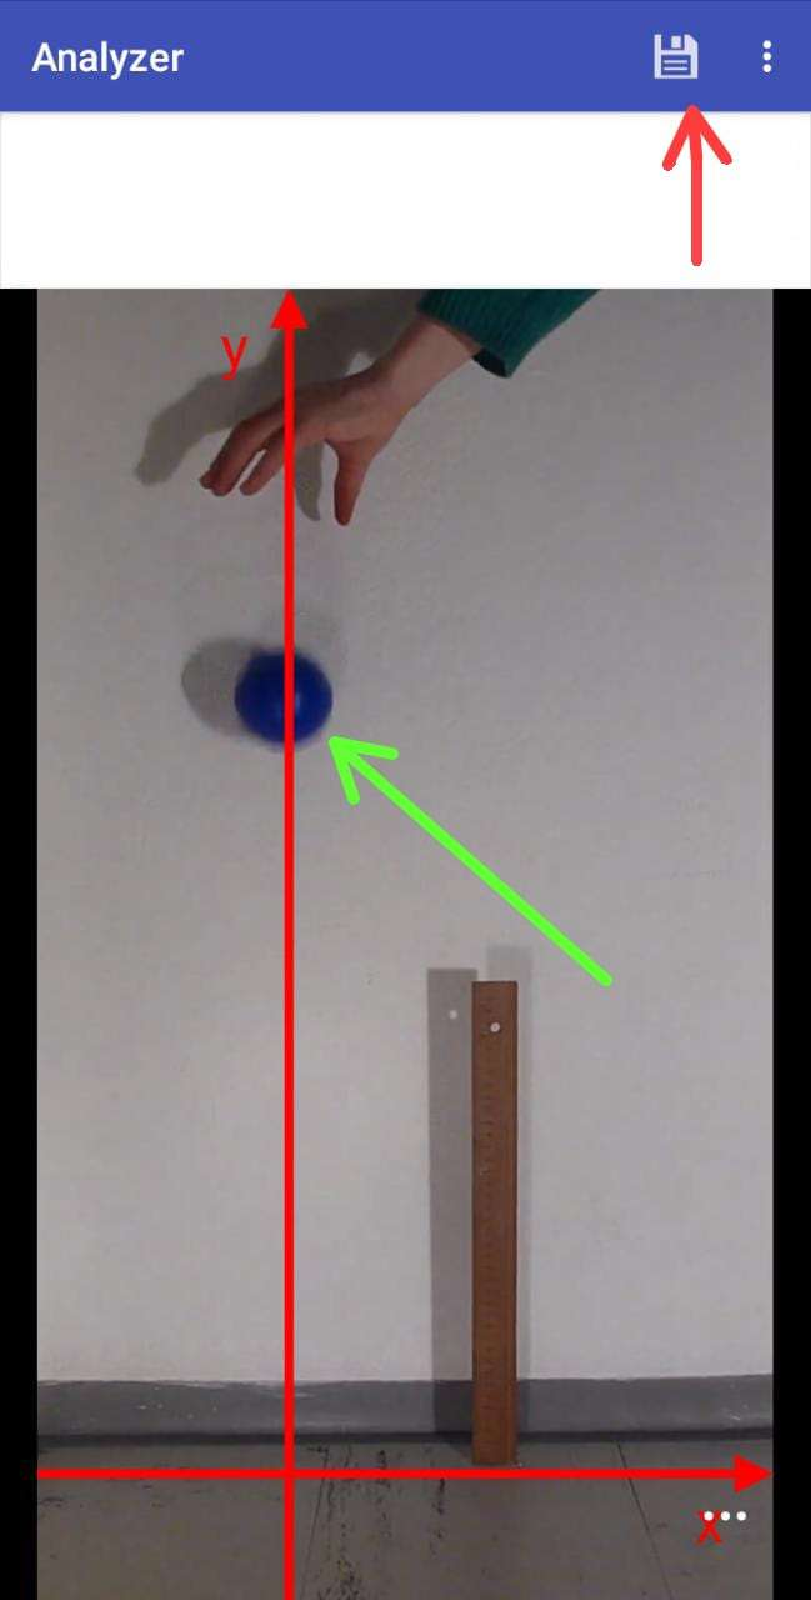
\includegraphics[width=8cm]{Figuras_exp3/imagenapendicec4.pdf}
\caption{\label{apendice4c} Sistema de eixos no reprodutor de vídeo do aplicativo VidAnalysis.}
\end{figure}


\underline{\bf Passo 3:} {\bf Coleta de dados}\\


A coleta de dados começa fazendo um ``click com o dedo no ponto do objeto que queremos seguir a trajetória, por exemplo no meio da bolinha azul na Figura~\ref{apendice4c}. Como as marcações são feitas com o dedo sugerimos que o corpo, cuja trajetória será determinada, seja suficientemente grande.
Depois que o primeiro ``click'' for feito, uma cruz azul aparecerá e o vídeo avançará alguns quadros. O intervalo de tempo transcorrido, medido em segundos, entre um ``click e outro e automaticamente determinado pelo programa. Vamos fazer ``click'' novamente tantas vezes como seja necessário para acompanhar a evolução da posição do objeto entre a posição inicial e final previamente estabelecidas. Leve em conta que para uma bolinha em queda vertical uma distância percorrida de um metro é o mínimo necessário para efetuar a análise, mas também não é necessário acompanhar 
todo o movimento do corpo até o chão.
\par 
Como mostrado na  Figura\ref{fig:reguacomxis},  pode ser que ao longo da trajetória não vejamos o corpo em questão claramente definido em uma única posição, mas como uma imagem embaçada devido à alta velocidade do mesmo. Então para determinar a posição do centro da bolinha e a sua incerteza siga as orientações indicadas nessa figura e no texto ao lado dela. 


\underline{\bf Passo 4:} {\bf Salvar dados}\\

Depois de determinados todos os pontos da trajetória do corpo, basta pressionar o botão ``Salvar', conforme mostrado pela seta vermelha na Figura~\ref{apendice4c}. Após o ``click'' se abrirá uma janela 
com a frase ``Nome para a análise'' (``Name for analysis'' em inglês). Uma vez escrito o nome do arquivo de dados dê ``click em ``ok'' e imediatamente verá uma janela na qual você poderá navegar. 
Rolando a imagem, no final aparecerá uma tabela com várias colunas de dados como mostrada na Figura \ref{apendice5c}.
É possível também exportar essa tabela de dados  para um arquivo que é uma planilha no formato ``.cvs'' (``comma separated values'''), que poderá ser lida por um programa de computador do tipo Excel. Mas também você poderá simplesmente copiar os dados que precisará (por exemplo 
a posição ``$y$'' como funçao do tempo ``$t$') numa folha de papel para continuar a análise. 
\par
Note que uma vez escolhido o nome do arquivo para a tabela de dados, esta tabela é automaticamente guardada pelo aplicativo. 
Para cada vídeo guardado dentro do aplicativo é possível realizar 
diferentes análises de dados e guardar cada um deles, dentro do aplicativo, 
com nomes diferentes.
Assim, por exemplo, na Figura~\ref{apendice1c} vemos vários vídeos guardados.
Se algum desses vídeos já foi analisado, quando fizer ``click nele aparecerá uma janela com 
várias opções de escolha. A primeira diz ``Começar análises'' (``Start analysis'' em inglês), o que permitirá realizar uma nova tomada de dados. Embaixo aparecem as outras opções que são
os nomes dos diferentes arquivos de dados já guardados. Fazendo ``click'' num deles é possível visualizar seu conteúdo novamente. Note que desta maneira é possível guardar a trajetória de mais de uma massa cujo movimento estiver gravado no vídeo. Assim, por exemplo, no caso em que a colisão de dois ou mais corpos estiver gravada no vídeo, é possível guardar os dados da trajetória de cada um deles.  

\begin{figure}[h!]
\centering
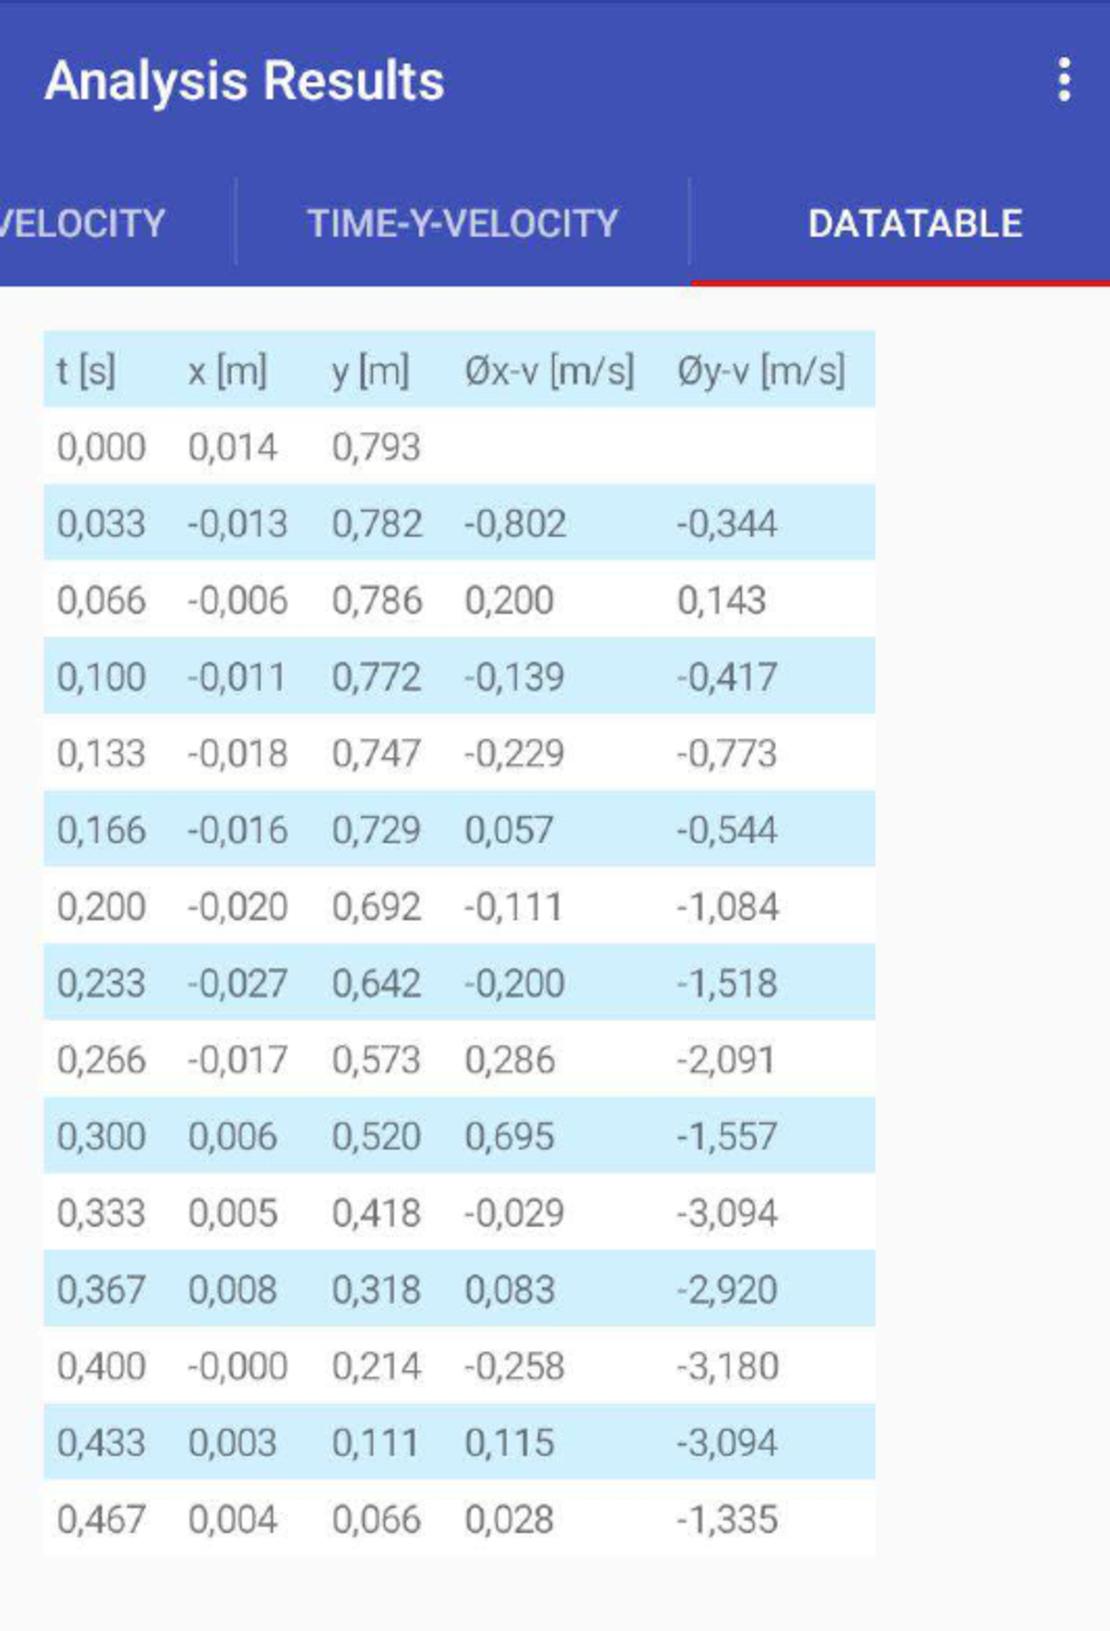
\includegraphics[width=8cm]{Figuras_exp3/imagenapendicec5.pdf}
\caption{\label{apendice5c} Tabela de dados gerada dentro do aplicativo VidAnalysis.}

\end{figure}